\phantomsection
\chapter{Developments in Machine Translation - Overview}

Machine Translation has a relatively brief history, comparable to that of modern computer science. It is the earliest application of Natural Language Processing using modern computers, that was conceived in the 1950s. However, the idea of using machines to assist translation isn't something new; The use of mechanical dictionaries in translation was first suggested in the 17th century\\ \cite{hutchins1992introduction}, and the techniques used for translation which are incorporated to produce a mechanized model of translation are even older, tracing back to 9th-century Arabic scholar named \textit{Al-Kindi}. His statistical observations and techniques for systematic translation produced results that even affected other domains of Computational Linguistics, such as authorship analysis and stylometrics \cite{dupont2018cryptological}.

In 1930, two patents were applied for mechanical bilingual dictionaries, one by French-Armenian Georges Artsrouni and another by a Russian Petr Troyanskii \cite{hutchins2001machine}. The latter held more importance as it proposed not only a method for a bilingual dictionary but also coding and interpreting grammatical functions using `universal' Esperanto-based symbols \cite{hutchins2005history}. However, the notion of using modern computers for translation originated from the depth of another research - cryptography. 

\phantomsection
\section{Cryptography, Translation \& Weaver}

Machine Translation was for a long time treated as a problem of cryptology \cite{dupont2018cryptological}. The origin of modern idea of the use of computers for Machine Translation can be traced back to Warren Weaver. In his discussions with Norbert Wiener, he presents his observations regarding the systematic encryption of language utterances into numbers using cryptographic techniques, which can then systematic-ally be decoded and return approximately the same original utterance, even if decoded by a person who doesn't know the language, as observed in cryptography \\ \cite{locke1954mechanical}. His perspective could be surmised by an excerpt from his letters to Wiener -

\begin{quote}
    One naturally wonders if the problem of translation could conceivably be treated as a problem in cryptography. When I look at an article in Russian, I say: `This is really written in English, but it has been coded in some strange symbols. I will now proceed to decode.'
\end{quote}

It was in his memorandum titled `Translation' in July 1949, that Weaver proposed his ideas, and presented his views on Machine Translation and the use of computers, statistics, and even neural networks for the purpose of translation \cite{hutchins1999warren}. This eventually became the driving force behind MT research in the 1950s, and its effects can be seen to date.

The memorandum first discussed the ongoing works and the progress made in the field. He put forward four proposals for further research in this field \cite{hutchins1999warren}.

\paragraph{Use of Context to Deal With Multiple Meanings} This idea could be surmised from -

\begin{quote}
    If one examines the words in a book, one at a time through an opaque mask with a hole in it one word wide, then it is obviously impossible to determine, one at a time, the meaning of words. ``Fast" may mean ``rapid"; or it may mean ``motionless"; and there is no way of telling which. But, if one lengthens the slit in the opaque mask, until one can see not only the central word in question but also say N words on either side, then, if N is large enough one can unambiguously decide the meaning. \cite{hutchins1999warren} \cite{weaver1952translation}
\end{quote}

\paragraph{Logical Elements in Language} In this proposal he brought attention to the research on mathematical modeling of neural structures of the human brain, and the use of such models in the form of robots or computers could be used to deduce any legitimate conclusion from a finite set of premises. This was under the assumption that there are logical elements in language \cite{weaver1952translation}.

\paragraph{Application of Cryptographical Methods} As discussed previously, Weaver put a lot of focus on the correlation between cryptography and translation, these ideas were primarily based on Information Theory, and the work he did with Claude Shannon \cite{hutchins1999warren}. He states -

\begin{quote}
    Frequencies of letters, letter combinations, intervals between letters and letter combinations, letter patterns, etc. which are to some significant degree independent of the language used.
\end{quote}

\paragraph{Linguistic Universals and Common Foundation for Languages} He pres-ented the notion that just like the presence of common logical features among languages, there might also by linguistics universals. In his analogy, he treats languages as towers with common basements, and that to communicate between languages one might need to descend to this common basement, i.e. the base of human communication derived by the extraction of logical features and identification of linguistic universals.

\cite{hutchins1999warren} notes that, in long term the most significant outcome of Weaver's memorandum was the appointment of logician Yehoshua Bar-Hillel to a research position at MIT (Massachusetts Institute of Technology) in 1951, which eventually led to the convening of the first conference in Machine Translation.

\phantomsection
\section{The First Generation}

The first MT conference produced great outcomes, where different scholars, discussed the direction of future research. Some of the highlights of the conference included the proposals for dealing with syntax by Oswald the Bar-Hilel, presenting arguments for a sublanguage system specifically for the purpose of translation \cite{hutchins1995machine}. 

The outcome of the conference made it obvious, that fully automatic translation would not be achievable without long-term basic research, and that in the meantime human assistance was needed for pre-editing and post-editing, i.e., preparing the SL text for translation and editing the output result to receive acceptable transla-tions \cite{reifler1952first}. There was also a discussion on the idea of a fulcrum language, a language as a point of leverage, to which and from other languages can be translated, which was discussed to be English \cite{reifler1952first}. The first requirement that numerous participants considered was a demonstration of the feasibility of Machine Translation \cite{hutchins1995machine}.

This was achieved with the Georgetown-IBM \cite{hutchins2004georgetown} experiment system in 1954, though the system was not one with practical feasibility, with only a sample of 49 carefully selected Russian sentences translated to English, with a vocabulary of only 250 words, using just 6 grammatical rules \cite{hutchins1995machine}. Yet, it achieved what it was meant to, to stimulate interest and garner large-scale funding. This also led to the rise of interest in MT in USSR \cite{hutchins1995machine}.

The research that followed either a trial-and-error based statistical approach to produce working systems (\textit{brute-force}), or a long-term solution-based theoretical approach, investing in fundamental linguistic research (\textit{perfectionist}) \cite{hutchins1995machine}. There was several works going on under different institutions in USA, as well as around the world. This was the time of Rule-Based Machine Translation. Well-known approaches were developed, `direct translation' which focuses on translation from a specific SL to a specific TL with a minimal amount of analysis and syntactic processing, `interlingua' approach, which focuses on an intermediate language independent representation. There was the `transfer approach' using 3 stages analysis, transfer, and synthesis \cite{hutchins2023machine}. Down below we have the 1985 version of the Vauquois triangle \cite{vauquois1968survey}, illustrating possible approaches in MT.

\begin{figure}[h]
    \centering
    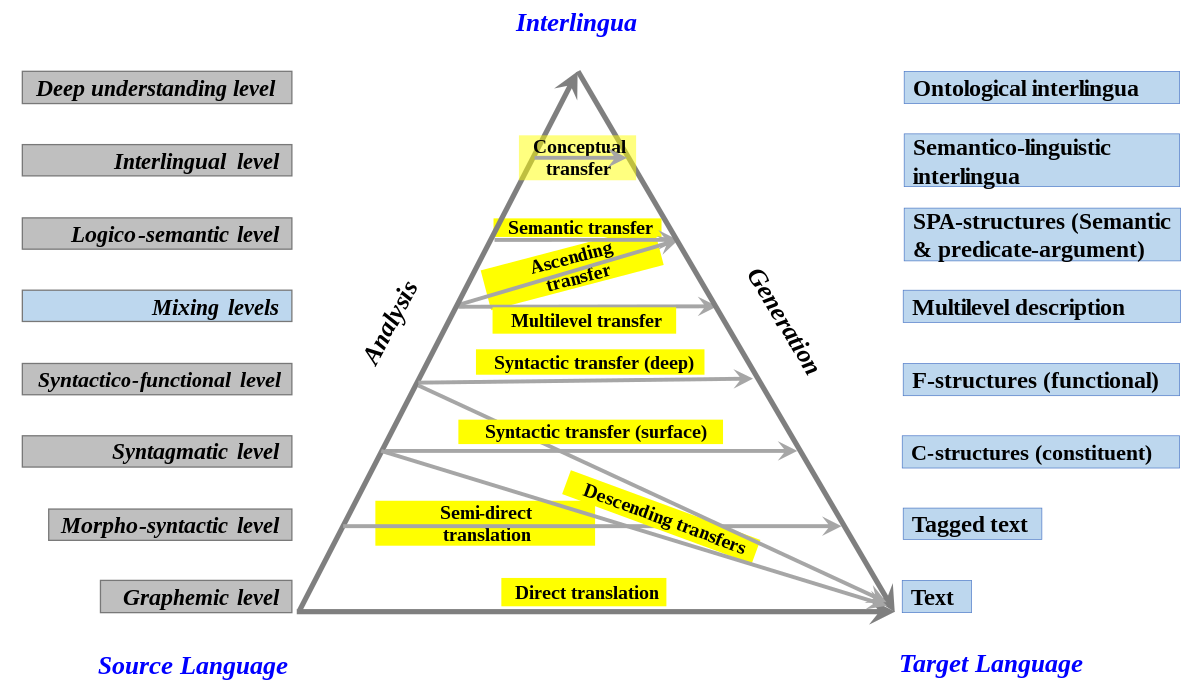
\includegraphics[width=\textwidth]{images/VauquoisModel.png}
    \caption{Vauquois triangle representing various MT approaches}
\end{figure}

Most of the research in MT, due to various reasons, hit a wall. With several institutions pulling out from the MT research altogether \cite{hutchins2023machine}, and the progress being too slow, it became a concern for the people putting in the funds.

\phantomsection
\section{ALPAC Report 1966 \& it's aftermath}

The US government sponsors becoming increasingly concerned about the lack of progress in Machine Translation, formed the Automatic Language Processing Advisory Committee (ALPAC) in 1964, which presented its first report in 1966. The report concluded that Machine Translation was twice as expensive as human translation, whereas slower, and less accurate, and that there was no predictable prospect for a useful machine translation system. It recommended that the focus be shifted to developing machine aids for human translators, such as mechanical bilingual dictionaries and other fundamental research in Computational Linguistics \cite{hutchins2023machine}. It saw no need to fund further MT research.

It had a great impact on the development of MT throughout the world, practically stagnating research in the United States for years. However, the research did not completely stop. Machine translation research just shifted direction. The new focus shifted to ``indirect" models: `interlingua' (translate text into a neutral intermediate language before converting it to the target language) and `transfer' based (analyze source and target languages separately, then transfer information for generation) \cite{hutchins2023machine}.

Examples of research projects in the 1970s and 1980s include the TAUM project (Montreal), which was successful with a syntactic transfer system for weather forecasts but struggled with complex phrases in other domains \cite{hutchins1995machine}. Another example is the ITS system (Brigham Young), which was abandoned due to complexity after a decade of development. A key trend in the 1980s was the emphasis on advanced methods and specific domains. Interlingua and transfer-based approaches continued to be explored alongside knowledge-based systems \cite{hutchins2023machine}. 

Research projects also expanded beyond North America, Western Europe, and Japan. The rise of operational machine translation systems included mainframe systems like Systran and microcomputer-based systems offered by companies like ALPS and Globalink \cite{hutchins1995machine}.

The interlingua approach faced challenges with rigidity and information loss. However, there was a renewed interest in the late 1980s with projects like DLT (Netherlands) and Rosetta (Netherlands). The transfer-based approach had influe-ntial projects like the GETA-Ariane system (Grenoble), which served as a model for many projects in the 1980s. Other notable projects included Mu (Kyoto University), SUSY (Saarbrücken), and Eurotra (European Communities) \\ \cite{hutchins2023machine}.

Knowledge-based approaches gained traction with projects in Japan, Europe, and North America. Overall, machine translation research diversified after the ALPAC report. The focus shifted to indirect models with an emphasis on practical applications. The 1980s also saw the rise of operational machine translation systems, along with the beginnings of speech translation research \cite{hutchins2023machine}.

\phantomsection
\section{Rise of Corpus-Based MT}

Till late 1980s, the field of Machine Translation was primarily dominated by the RBMT approaches, be it knowledge-based systems, or linguistics based. However, this dominance was broken in 1989, with the emergence of corpus-based methods. It began with the Candide project at IMB, which revived the long-forgotten statistics-based approach, which was suggested by Weaver and was one of the earlier approaches studied \cite{yang2014statistical} \cite{hutchins2023machine}. 

The Candide system was tested on a large corpus of French and English texts contained in the reports of Canadian parliamentary debates. The results were surprising, nearly half the translated phrases matched the exact translation present in the corpus or resulted in translations with words that presented the same sense, or any other acceptable translations \cite{berger1994candide} \cite{hutchins2023machine}.

\phantomsection
\paragraph{Statistical Machine Translation (SMT)}
SMT generates translations based on a probabilistic model of the translation process, the parameters of which are estimated from parallel text. Unlike RBMT approaches, which require one to extract and develop rules manually and are hard to generalize to other languages, SMT on the other hand pursuers a data-driven approach and derives the translation knowledge from the corpora \cite{yang2014statistical}.

SMT has 3 fundamental problems that need to be addressed - \textit{modeling} (the probabilistic modeling of the translation process), \textit{training} (deals with learning the required translation knowledge i.e. estimating required parameters), and \textit{decoding} (finding the target language text with maximum probability in a reasonable amount of time) \cite{yang2014statistical}.

SMT can be categorized into rule-based, phrase-based, and syntax-based appro-aches \cite{yang2014statistical}.

\phantomsection
\paragraph{Example-Based Machine Translation (EBMT)}

EBMT was another corpus-based translation approach. It relies on large databases of translated texts, and works by finding similar phrases or sentences in the database that have already been translated by humans and using those translations as a guide for the new text. This approach is based on the idea that human translators often reuse past translations, and EBMT tries to replicate this behavior. This approach was first proposed by Makato Nagao \cite{nagao1984framework}. Nagao States -

\begin{quote}
    Man does not translate a simple sentence by doing deep linguistic analysis, rather, man does the translation, first, by properly decomposing an input sentence into certain fragmental phrases … then by translating these phrases into other language phrases, and finally by properly composing these fragmental translations into one long sentence. The translation of each fragmental phrase will be done by the analogy translation principle with proper examples as its reference.
\end{quote}

The three main components of EBMT are - matching source fragments against the examples, identifying the corresponding translation fragments, and then recom-bining them to give the target output \cite{wong2023example}.

With the emergence of personal computers, and the involvement of many companies such as Google, Machine Translation became available for the general public, and SMT was the most prevalent MT approach used by them. It remained so, till the early 2010s when Neural Machine Translation came into the picture.

\phantomsection
\section{Neural Machine Translation}

The idea of using neural networks for the purpose of translation was discussed way back in the 1980s \cite{allen1987several}, though it didn't have much of a presence until the early 2010s. In 2013, a paper by Kalchbrenner \& Blunsom \\ \cite{kalchbrenner2013recurrent} showed the use of Convolutional Neural Networks (CNN) for encoding the source and then using it for translation, on the other hand, two papers by Cho et. al. \cite{cho2014learning} and Sutskever et. al. \cite{sutskever2014sequence} in 2014, made use of Recurrent Neural Network (RNN) for the same. 

It was Cho et. al. \cite{cho2014learning} that proposed the RNN-based Encoder-Decoder architecture the foundation for a lot of AI applications to date. In this architecture, the encoder maps a variable length source sequence to a fixed length vector, which is then mapped to a variable length target sequence by the decoder (Fig \ref{fig:encode-decode}). Sutskever et. al. \cite{sutskever2014sequence} used LSTM (Long Short-Term Memory) in place of traditional RNNs. They observed a BLEU score of 36.5, for reference, the model proposed by Kalchbrenner \& Blunsom \cite{kalchbrenner2013recurrent} had a BLEU score of around 21.8.

These produced acceptable results in short-length sentences but performed poorly when dealing with longer-length sentences. A solution to this problem was proposed by Bahdanau et. al. \cite{bahdanau2014neural} in form of the `\textit{attention}' mechanism. This mechanism computes a context vector $ c_i $ as a weighted sum of annotations $ h_j $ of the source sentence \cite{bahdanau2014neural}. The weight $ \alpha_{ij} $  of each annotation  $ h_j $  is determined by an alignment model $ e_{ij} = a(s_{i-1}, h_j) $, which scores how well the inputs around position $ j $ and the output at position $ i $ match \cite{bahdanau2014neural}. This allows the model to selectively focus on relevant parts of the source sentence when generating each target word \cite{bahdanau2014neural}.

These developments made NMT the primary area of focus in the field of Machine Translation. These developments led to the launch of first large-scale NMT model by Baidu \cite{he2015baidu} in the year 2015, followed by Google in 2016 \cite{wu2016google}. DeepL was launched in 2017, and used CNN to encode sentences at that time \cite{schmitt2019translation}.

2017 was also the year when Vaswani et. al. published the paper titled `\textit{Attention Is All You Need}' \cite{vaswani2017attention}. This paper introduced us to the \textit{Transformers} architecture, and the concept of self-attention, which was applied to all the steps in the encoder-decoder architecture \cite{vaswani2017attention}. Self-attention, also known as intra-attention, is a mechanism that allows a model to relate different positions within a single sequence to compute a representation of that sequence \cite{vaswani2017attention}. This architecture produced a BLEU score of 41.0 on WMT 2014 English-French with training for just 3.5 days on 8 GPUs \cite{vaswani2017attention}. The architecture proposed was highly parallelizable, signifi-cantly reducing training time and capturing long-range dependencies. Though this architecture was developed for NMT, its aforementioned characteristics allowed for its application in many domains, and also led to the emergence of Large Language Models (LLMs).

In 2018 two Large Language Models were released - \gls{bert} \cite{devlin2018bert} by Google and \gls{gpt} \cite{radford2018improving} by OpenAI. These models and other pre-trained LLMs following them could be fine-tuned for various applications, one of those applications is Translation. The Generative LLMs developed later can also be prompted to translate the provided text \\ \cite{klamra2023evaluating}. LLMs also show promising levels of performance in translation, as they are able to handle various contextual information such as cultural nuances, etc. \cite{yao2023empowering}. Though generative and conversational LLMs can be used for translation, modern NMT systems still use the sequence-to-sequence translation model as proposed by \cite{sutskever2014sequence}.